\chapter{Theoretical background}

\section{Distributions}
\subsection{Poisson distribution}
One very important probability distribution in physics is the Poisson
distribution. It describes the results of ``counting experiments'' and is
therefore very important for image processing as the pictures taken with a
camera are in principle counts of photons reaching the camera. Photon counting
noise is one important example.\\
Poisson distributions are just defined for integer values and the variance is
the same as the mean value of the distribution. Another important attribute is
the skewnes which is the inverse of the squarerot of the mean or variance and describes the assymetry.\\ 
The probability mass function is:
\begin{equation}
	p(n,\mu) = \frac{\mu^n}{n!}\exp(-\mu)
\end{equation}
\subsection{Skellam distribution}
The probability
mass function of a Skellam distribution is a function of the difference between
two Poisson random variables
\begin{equation}
	p(k;\mu_1, \mu_2) =
	\exp(-(\mu_1+\mu_2))\left(\frac{\mu_1}{\mu_2}\right)^{k/2}~I_{|k|}\left(2\sqrt{\mu_1
	\mu_2}\right)
\end{equation}  
where $n_1$, $n_2$ are the Poisson random variables and $k = n_1 - n_2$.
$I_{|k|}$ means the modified Bessel function of the first kind.\\
Mean $\mu$ and variance $\sigma$ of the Skellam distribution are given by
\begin{align}
	&&\mu &= \mu_1 - \mu_2,& \sigma^2 &= \mu_1 + \mu_2\\
	\Rightarrow &&\mu_1& = \frac{\mu + \sigma^2}{2},& \mu_2 &=\frac{-\mu +
	\sigma^2}{2}
\end{align} 

\subsection{Approach using skewness of poisson distribution}
For every pixel there is a set of multiple values in the set. This allows to
calculate the different parameters individually for each pixel. One can
calculate mean and variance of the measured intensities $I_\text{meas}(i,j)$ and
gets
\begin{align}
	\text{mean}(I_\text{meas}(i,j))& = g\cdot \text{mean}(I_\text{true}(i,j)) + o \label{meanvarPoiss1}\\
	\text{var}(I_\text{meas}(i,j))& = g^2\cdot\text{var}(I_\text{true}(i,j)) \label{meanvarPoiss2}
\end{align}
Assuming a Poisson distribution as the true intensity, mean and variance would
be the same. Unfortunately the mean true intensities are unknown and it is
not possible to determin $g$ and $o$ so far. For large mean Intensities $\mu$
the Poisson distribution becomes more and more similar to a Gauss distribution
with the same mean. However, for small means, the Poisson distribution is not
symmetric. The skewness $s_p$ of a Poission distribution is the inverse of the
square root of the mean $(\mu)^{-.5}$. It can also be directly
calculated from data
\begin{equation}
	s_p = \frac{1}{n}\sum_{i = 1}^n \left(\frac{x_i - \bar x}{\sigma}\right)^3
\end{equation}
The skewness is invariant to shift and multiplication with a constant. This
means that the transformation caused by the camera gain and the dark current
does not affect the skewness. This gives a third equation to solve for $g$ and
$o$.\\
This approach has very strict limitation at least for background pixels not to be too
bright. If the mean of the true Poisson distributin is higher than
roughly 30 the skewness gives due to noise no stabel results and it is
impossible to determin the mean intensity in this way.


\section{the data}
The concept of direct stochastic optical reconstruction microscopy (dSTORM) \cite{heilemann} is, to label interesting structures with fluorophors that can be exited using a laser with the appropriate wavelength. After a short time the flourophors emit a photon and go back to the unexited state or lose the ability to get exited, they bleach out.
The datasets for dSTORM microscopy that we recieve from our collaborators from
Bioquant are big datasets of several gigabyte in the Andor .sif format. Each
file conains a stack of pictures, normaly between 1000 and 10000, taken
consecutively with exposure times between 20 and 200 milliseconds.\newline

Picture /ref{rawStorm} shows a typical frame of raw data. In each frame there might be multiple flourophores visible at the same time. Due to the large magnification, beyond the diffraction limit, the almost pointlike flourophores appear as gaussian shaped signals, their point spread functions. The flourophores are either attached to the biological structures that are of interest or they form a cluster, called a bead.\newline

Beads are larger and brighter than spots form only one flourophore and are used to align multiple channels in the postprocessing step. Beads are designt to show up in every frame of the sequence at the same position. They are composed of flourophores of different color to be visible in every channel.\newline

The other spots, bound to some proteins for example, are just lighting up for a very short time. This is the key aspect of dSTORM. Instead of one frame that shows all flourophores at the same time, thousands of frames are captured containing just a point spread functions per frame. This gives the possibility to determine the center of each point spread function with sub-pixel precision, and in the end when all points are displayed together in one picture, to an image with a resolution beyond the diffraction limit.

\begin{figure}
\centering
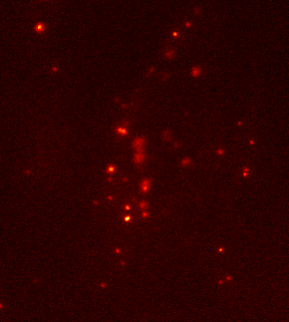
\includegraphics[width = 0.88\textwidth]{pictures/Pos2_2_red2-2frame2475Color.png}
	\caption{Raw image for dSTORM processing}
	\label{rawStorm}
\end{figure}


\section{Transformations}
\subsection{Transformation to Poisson distributed signal} \label{trafoPoiss}
The images aquired from the camera show not the real intensities
$I_\text{true}$, which result from the photon emission of the probe, but
transformed ones $I_\text{meas}$. I consider two main reasons why the taken image
differs from the true image, besides noise.\\
There is dark current which means that even a picture taken with closed shutter
would get some intensity, even without any light hitting the sensor chip of the
camera. This is a result of thermal movement of the atoms off the sensor chip
and can be reduced by cooling. The dark current noise adds an almost constant
value $o$ to the output signal.
Incoming photons create electrons via inner photoelectric effect. This electrons
are collected for each pixel and might be amplified to get the final result.
Assuming a linear relation between the number of incoming photons and the number
of electrons created and a linear amplifier results in a factor $g$. This factor
is multiplied with the number of photons captured during exposure time for each
pixel.\\
If the gain factor $g$ and the offset $o$ are known the true intensity, the
number of photons detected is:
\begin{equation}
	I_\text{true} = \dfrac{I_\text{meas}-o}{g}. \label{transtopoiss}
\end{equation}
\subsection{Anscombe transformation}
\label{trafoAnscombe}
The Anscombe transform is used to transform a random variable with a Poisson
distribution into one with an approximatly constant standard deviation. The
transformation is defined as:
\begin{equation}
	A(x) = 2\sqrt{x+\frac{3}{8}}.
\end{equation}
As one can see in figure \ref{anscombe} the Anscombe transformations result has
for mean intensities greater than 4 a intensity independent standard deviation of
one.
\begin{figure}
	\centering
	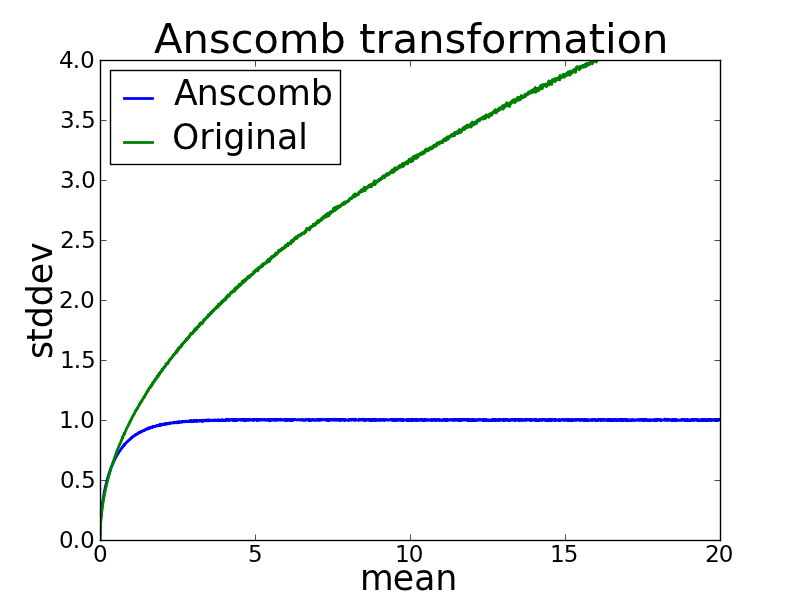
\includegraphics[width = 0.5\textwidth]{pictures/anscombe.png}
	\caption{Standard deviation over mean intensities of different Poisson
	distributions}
	\label{anscombe}
	
\end{figure}

\section{Estimation of camera gain}
Given a sample prepared for STORM microscopy. A sequence of images captured from this sample will show some active flourophores, beads and also illuminated background that comes from flourophores that lie not in the focus plane. Assuming an inhomogenous background signal that follows a Poisson distribution, or even better almost homogenous background and beads both with a Poisson distribution in time with different mean values. If this Signal $I_\text{true}$ is transformed in the following way:
\begin{equation}
	I_\text{meas} = g \cdot I_\text{true} + o \label{trafoGain}
\end{equation}
This is the inverse transformation of equatione \ref{transtopoiss}.\newline
Considering two pixels with different Poisson distributions $P_1$ and $P_2$ with mean value and variances of this distributions $\lambda_1$ and $\lambda_2$. If this distributions are transfomed as given in equation \ref{trafoGain} their mean and variance change like shown in equation \ref{meanvarPoiss1} and \ref{meanvarPoiss2}. This gives the oportunity to determine the gain and offset using two or more pixels.
\begin{align}
	\text{var}(I_{\text{meas}1})& = g^2\cdot\text{var}(I_{\text{true}1})\\ 
	\text{var}(I_{\text{meas}2})& = g^2\cdot\text{var}(I_{\text{true}2})\\
	\text{mean}(I_{\text{meas}1})& = g\cdot \text{mean}(I_{\text{true}1}) + o\\
	\text{mean}(I_{\text{meas}2})& = g\cdot \text{mean}(I_{\text{true}2}) + o
\end{align}
The values for $\text{var}(I_{\text{meas}1/2})$ and $\text{mean}(I_{\text{true}1/2})$ can be calculated from the data and can be used to get the gain as follows:
\begin{align}
	\frac{\text{var}(I_{\text{meas}1})-\text{var}(I_{\text{meas}2})}{\text{mean}({\text{meas}1})-\text{mean}(I_{\text{meas}2})}&= \frac{g^2\cdot \lambda_1  - g^2\cdot \lambda_2 }{g\cdot \lambda_1 + o - (g\cdot \lambda_2+o)}\\
	& = \frac{g^2\cdot(\lambda_1-\lambda_2)}{g\cdot (\lambda_1-\lambda_2)}\\
	& = g
\end{align}
In the same manner the offset $o$ can be calculated.
\begin{align}
	\text{mean}(I_{\text{meas}1}) - \frac{\text{var}(I_{\text{meas}1})}{g} &= g\cdot \lambda_1 + o - \frac{g^2\cdot\lambda_1}{g}\\
	&= o
\end{align}


